\hypertarget{LinearStatistic_8c}{
\section{Linear\-Statistic.c File Reference}
\label{LinearStatistic_8c}\index{LinearStatistic.c@{LinearStatistic.c}}
}
{\tt \#include \char`\"{}CI\_\-common.h\char`\"{}}\par


Include dependency graph for Linear\-Statistic.c:\begin{figure}[H]
\begin{center}
\leavevmode
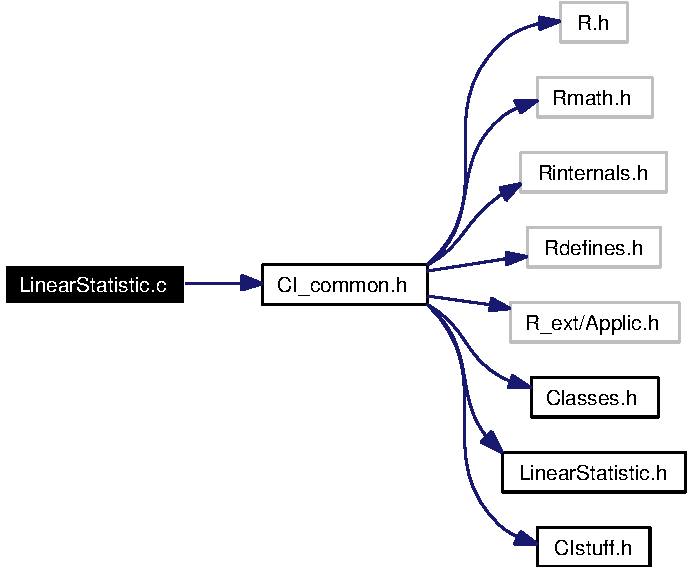
\includegraphics[width=186pt]{LinearStatistic_8c__incl}
\end{center}
\end{figure}
\subsection*{Functions}
\begin{CompactItemize}
\item 
void \hyperlink{LinearStatistic_8c_a0}{C\_\-kronecker} (const double $\ast$A, const int m, const int n, const double $\ast$B, const int r, const int s, double $\ast$ans)
\item 
SEXP \hyperlink{LinearStatistic_8c_a1}{R\_\-kronecker} (SEXP A, SEXP B)
\item 
void \hyperlink{LinearStatistic_8c_a2}{C\_\-Expect\-Covar\-Influence} (const double $\ast$y, const int q, const double $\ast$weights, const int n, SEXP ans)
\item 
SEXP \hyperlink{LinearStatistic_8c_a3}{R\_\-Expect\-Covar\-Influence} (SEXP y, SEXP weights)
\item 
void \hyperlink{LinearStatistic_8c_a4}{C\_\-Expect\-Covar\-Linear\-Statistic} (const double $\ast$x, const int p, const double $\ast$y, const int q, const double $\ast$weights, const int n, const SEXP expcovinf, SEXP ans)
\item 
SEXP \hyperlink{LinearStatistic_8c_a5}{R\_\-Expect\-Covar\-Linear\-Statistic} (SEXP x, SEXP y, SEXP weights, SEXP expcovinf)
\item 
void \hyperlink{LinearStatistic_8c_a6}{C\_\-Linear\-Statistic} (const double $\ast$x, const int p, const double $\ast$y, const int q, const double $\ast$weights, const int n, double $\ast$ans)
\item 
SEXP \hyperlink{LinearStatistic_8c_a7}{R\_\-Linear\-Statistic} (SEXP x, SEXP y, SEXP weights)
\item 
void \hyperlink{LinearStatistic_8c_a8}{C\_\-Permuted\-Linear\-Statistic} (const double $\ast$x, const int p, const double $\ast$y, const int q, const int n, const int nperm, const int $\ast$indx, const int $\ast$perm, double $\ast$ans)
\item 
SEXP \hyperlink{LinearStatistic_8c_a9}{R\_\-Permuted\-Linear\-Statistic} (SEXP x, SEXP y, SEXP indx, SEXP perm)
\item 
void \hyperlink{LinearStatistic_8c_a10}{C\_\-scmatleft} (const double $\ast$x, const int p, const int q, double $\ast$ans)
\item 
SEXP \hyperlink{LinearStatistic_8c_a11}{R\_\-scmatleft} (SEXP x, SEXP pq)
\item 
void \hyperlink{LinearStatistic_8c_a12}{C\_\-scmatright} (const double $\ast$x, const int p, const int q, double $\ast$ans)
\item 
SEXP \hyperlink{LinearStatistic_8c_a13}{R\_\-scmatright} (SEXP x, SEXP pq)
\end{CompactItemize}


\subsection{Detailed Description}
Linear statistics for conditional inference

\begin{Desc}
\item[Author:]\begin{Desc}
\item[Author]hothorn \end{Desc}
\end{Desc}
\begin{Desc}
\item[Date:]\begin{Desc}
\item[Date]2005/10/13 12:45:01 \end{Desc}
\end{Desc}


Definition in file \hyperlink{LinearStatistic_8c-source}{Linear\-Statistic.c}.

\subsection{Function Documentation}
\hypertarget{LinearStatistic_8c_a2}{
\index{LinearStatistic.c@{Linear\-Statistic.c}!C_ExpectCovarInfluence@{C\_\-ExpectCovarInfluence}}
\index{C_ExpectCovarInfluence@{C\_\-ExpectCovarInfluence}!LinearStatistic.c@{Linear\-Statistic.c}}
\subsubsection[C\_\-ExpectCovarInfluence]{\setlength{\rightskip}{0pt plus 5cm}void C\_\-Expect\-Covar\-Influence (const double $\ast$ {\em y}, const int {\em q}, const double $\ast$ {\em weights}, const int {\em n}, SEXP {\em ans})}}
\label{LinearStatistic_8c_a2}


Conditional expectation and covariance of the influence function\par
 \begin{Desc}
\item[Parameters:]
\begin{description}
\item[{\em y}]values of the influence function \item[{\em q}]dimension of the influence function \item[{\em weights}]case weights \item[{\em n}]number of observations \item[{\em ans}]return value; an object of class `Expect\-Covar\-Influence' \end{description}
\end{Desc}


Definition at line 80 of file Linear\-Statistic.c.

References CI\_\-covariance\-Sym, CI\_\-expectation\-Sym, and CI\_\-sumweights\-Sym.

Referenced by R\_\-Expect\-Covar\-Influence().\hypertarget{LinearStatistic_8c_a4}{
\index{LinearStatistic.c@{Linear\-Statistic.c}!C_ExpectCovarLinearStatistic@{C\_\-ExpectCovarLinearStatistic}}
\index{C_ExpectCovarLinearStatistic@{C\_\-ExpectCovarLinearStatistic}!LinearStatistic.c@{Linear\-Statistic.c}}
\subsubsection[C\_\-ExpectCovarLinearStatistic]{\setlength{\rightskip}{0pt plus 5cm}void C\_\-Expect\-Covar\-Linear\-Statistic (const double $\ast$ {\em x}, const int {\em p}, const double $\ast$ {\em y}, const int {\em q}, const double $\ast$ {\em weights}, const int {\em n}, const SEXP {\em expcovinf}, SEXP {\em ans})}}
\label{LinearStatistic_8c_a4}


Conditional expectation and covariance of the a linear statistic\par
 \begin{Desc}
\item[Parameters:]
\begin{description}
\item[{\em x}]values of the transformation \item[{\em p}]dimension of the transformation \item[{\em y}]values of the influence function \item[{\em q}]dimension of the influence function \item[{\em weights}]case weights \item[{\em n}]number of observations \item[{\em expcovinf}]an object of class `Expect\-Covar\-Influence' \item[{\em ans}]return value; an object of class `Expect\-Covar' \end{description}
\end{Desc}


Definition at line 192 of file Linear\-Statistic.c.

References C\_\-kronecker(), CI\_\-covariance\-Sym, CI\_\-expectation\-Sym, and CI\_\-sumweights\-Sym.

Referenced by R\_\-Expect\-Covar\-Linear\-Statistic().

Here is the call graph for this function:\begin{figure}[H]
\begin{center}
\leavevmode
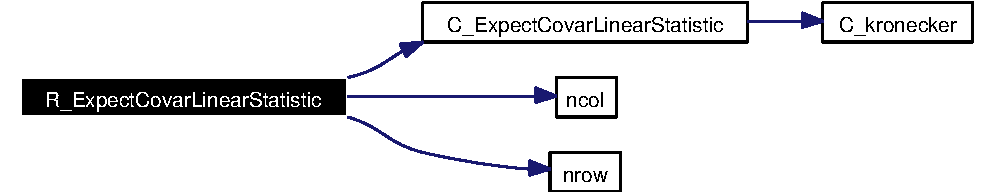
\includegraphics[width=158pt]{LinearStatistic_8c_a4_cgraph}
\end{center}
\end{figure}
\hypertarget{LinearStatistic_8c_a0}{
\index{LinearStatistic.c@{Linear\-Statistic.c}!C_kronecker@{C\_\-kronecker}}
\index{C_kronecker@{C\_\-kronecker}!LinearStatistic.c@{Linear\-Statistic.c}}
\subsubsection[C\_\-kronecker]{\setlength{\rightskip}{0pt plus 5cm}void C\_\-kronecker (const double $\ast$ {\em A}, const int {\em m}, const int {\em n}, const double $\ast$ {\em B}, const int {\em r}, const int {\em s}, double $\ast$ {\em ans})}}
\label{LinearStatistic_8c_a0}


Computes the Kronecker product of two matrices\par
 \begin{Desc}
\item[Parameters:]
\begin{description}
\item[{\em A}]matrix \item[{\em m}]nrow(A) \item[{\em n}]ncol(A) \item[{\em B}]matrix \item[{\em r}]nrow(B) \item[{\em s}]ncol(B) \item[{\em ans}]return value; a pointer to a REALSXP-vector of length (mr x ns) \end{description}
\end{Desc}


Definition at line 22 of file Linear\-Statistic.c.

Referenced by C\_\-Expect\-Covar\-Linear\-Statistic(), and R\_\-kronecker().\hypertarget{LinearStatistic_8c_a6}{
\index{LinearStatistic.c@{Linear\-Statistic.c}!C_LinearStatistic@{C\_\-LinearStatistic}}
\index{C_LinearStatistic@{C\_\-LinearStatistic}!LinearStatistic.c@{Linear\-Statistic.c}}
\subsubsection[C\_\-LinearStatistic]{\setlength{\rightskip}{0pt plus 5cm}void C\_\-Linear\-Statistic (const double $\ast$ {\em x}, const int {\em p}, const double $\ast$ {\em y}, const int {\em q}, const double $\ast$ {\em weights}, const int {\em n}, double $\ast$ {\em ans})}}
\label{LinearStatistic_8c_a6}


Computes the linear statistic, formula (1) in the paper\par
 \begin{Desc}
\item[Parameters:]
\begin{description}
\item[{\em x}]values of the transformation \item[{\em p}]dimension of the transformation \item[{\em y}]values of the influence function \item[{\em q}]dimension of the influence function \item[{\em weights}]case weights \item[{\em n}]number of observations \item[{\em ans}]return value; a pointer to a REALSXP-vector of length pq \end{description}
\end{Desc}


Definition at line 327 of file Linear\-Statistic.c.

Referenced by R\_\-Linear\-Statistic().\hypertarget{LinearStatistic_8c_a8}{
\index{LinearStatistic.c@{Linear\-Statistic.c}!C_PermutedLinearStatistic@{C\_\-PermutedLinearStatistic}}
\index{C_PermutedLinearStatistic@{C\_\-PermutedLinearStatistic}!LinearStatistic.c@{Linear\-Statistic.c}}
\subsubsection[C\_\-PermutedLinearStatistic]{\setlength{\rightskip}{0pt plus 5cm}void C\_\-Permuted\-Linear\-Statistic (const double $\ast$ {\em x}, const int {\em p}, const double $\ast$ {\em y}, const int {\em q}, const int {\em n}, const int {\em nperm}, const int $\ast$ {\em indx}, const int $\ast$ {\em perm}, double $\ast$ {\em ans})}}
\label{LinearStatistic_8c_a8}


Linear Statistic with permuted indices\par
 \begin{Desc}
\item[Parameters:]
\begin{description}
\item[{\em x}]values of the transformation \item[{\em p}]dimension of the transformation \item[{\em y}]values of the influence function \item[{\em q}]dimension of the influence function \item[{\em n}]number of observations \item[{\em nperm}]number of permutations \item[{\em indx}]indices for the x-part \item[{\em perm}](permuted) indices for the y-part \item[{\em ans}]return value; a pointer to a REALSXP-vector of length pq \end{description}
\end{Desc}


Definition at line 409 of file Linear\-Statistic.c.

Referenced by R\_\-Monte\-Carlo\-Independence\-Test(), and R\_\-Permuted\-Linear\-Statistic().\hypertarget{LinearStatistic_8c_a10}{
\index{LinearStatistic.c@{Linear\-Statistic.c}!C_scmatleft@{C\_\-scmatleft}}
\index{C_scmatleft@{C\_\-scmatleft}!LinearStatistic.c@{Linear\-Statistic.c}}
\subsubsection[C\_\-scmatleft]{\setlength{\rightskip}{0pt plus 5cm}void C\_\-scmatleft (const double $\ast$ {\em x}, const int {\em p}, const int {\em q}, double $\ast$ {\em ans})}}
\label{LinearStatistic_8c_a10}


Score matrix for a linear combination of a linear statistic from the left\par
 \begin{Desc}
\item[Parameters:]
\begin{description}
\item[{\em x}]score vector of length p \item[{\em p}]length of x \item[{\em q}]dimension of the influence function \item[{\em ans}]return value; a pointer to a q x (pq) matrix \end{description}
\end{Desc}


Definition at line 498 of file Linear\-Statistic.c.

Referenced by R\_\-scmatleft().\hypertarget{LinearStatistic_8c_a12}{
\index{LinearStatistic.c@{Linear\-Statistic.c}!C_scmatright@{C\_\-scmatright}}
\index{C_scmatright@{C\_\-scmatright}!LinearStatistic.c@{Linear\-Statistic.c}}
\subsubsection[C\_\-scmatright]{\setlength{\rightskip}{0pt plus 5cm}void C\_\-scmatright (const double $\ast$ {\em x}, const int {\em p}, const int {\em q}, double $\ast$ {\em ans})}}
\label{LinearStatistic_8c_a12}


Score matrix for a linear combination of a linear statistic from the right\par
 \begin{Desc}
\item[Parameters:]
\begin{description}
\item[{\em x}]score vector of length q \item[{\em p}]dimension of the transformation \item[{\em q}]length of x \item[{\em ans}]return value; a pointer to a p x (pq) matrix \end{description}
\end{Desc}


Definition at line 563 of file Linear\-Statistic.c.

Referenced by R\_\-scmatright().\hypertarget{LinearStatistic_8c_a3}{
\index{LinearStatistic.c@{Linear\-Statistic.c}!R_ExpectCovarInfluence@{R\_\-ExpectCovarInfluence}}
\index{R_ExpectCovarInfluence@{R\_\-ExpectCovarInfluence}!LinearStatistic.c@{Linear\-Statistic.c}}
\subsubsection[R\_\-ExpectCovarInfluence]{\setlength{\rightskip}{0pt plus 5cm}SEXP R\_\-Expect\-Covar\-Influence (SEXP {\em y}, SEXP {\em weights})}}
\label{LinearStatistic_8c_a3}


R-interface to C\_\-Expect\-Covar\-Influence\par
 \begin{Desc}
\item[Parameters:]
\begin{description}
\item[{\em y}]values of the influence function \item[{\em weights}]case weights \end{description}
\end{Desc}


Definition at line 150 of file Linear\-Statistic.c.

References C\_\-Expect\-Covar\-Influence(), CI\_\-covariance\-Sym, CI\_\-expectation\-Sym, CI\_\-sumweights\-Sym, ncol(), and nrow().

Here is the call graph for this function:\begin{figure}[H]
\begin{center}
\leavevmode
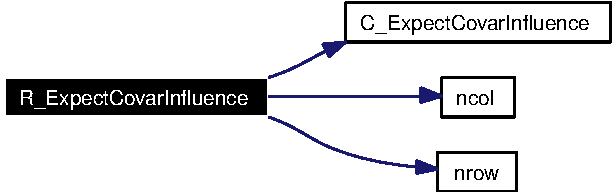
\includegraphics[width=179pt]{LinearStatistic_8c_a3_cgraph}
\end{center}
\end{figure}
\hypertarget{LinearStatistic_8c_a5}{
\index{LinearStatistic.c@{Linear\-Statistic.c}!R_ExpectCovarLinearStatistic@{R\_\-ExpectCovarLinearStatistic}}
\index{R_ExpectCovarLinearStatistic@{R\_\-ExpectCovarLinearStatistic}!LinearStatistic.c@{Linear\-Statistic.c}}
\subsubsection[R\_\-ExpectCovarLinearStatistic]{\setlength{\rightskip}{0pt plus 5cm}SEXP R\_\-Expect\-Covar\-Linear\-Statistic (SEXP {\em x}, SEXP {\em y}, SEXP {\em weights}, SEXP {\em expcovinf})}}
\label{LinearStatistic_8c_a5}


R-interface to C\_\-Expect\-Covar\-Linear\-Statistic\par
 \begin{Desc}
\item[Parameters:]
\begin{description}
\item[{\em x}]values of the transformation \item[{\em y}]values of the influence function \item[{\em weights}]case weights \item[{\em expcovinf}]an object of class `Expect\-Covar\-Influence' \end{description}
\end{Desc}


Definition at line 285 of file Linear\-Statistic.c.

References C\_\-Expect\-Covar\-Linear\-Statistic(), CI\_\-covariance\-Sym, CI\_\-expectation\-Sym, ncol(), and nrow().

Here is the call graph for this function:\begin{figure}[H]
\begin{center}
\leavevmode
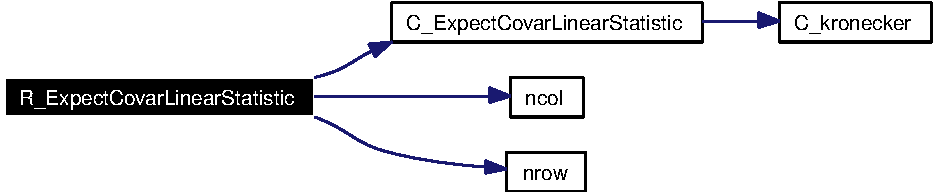
\includegraphics[width=255pt]{LinearStatistic_8c_a5_cgraph}
\end{center}
\end{figure}
\hypertarget{LinearStatistic_8c_a1}{
\index{LinearStatistic.c@{Linear\-Statistic.c}!R_kronecker@{R\_\-kronecker}}
\index{R_kronecker@{R\_\-kronecker}!LinearStatistic.c@{Linear\-Statistic.c}}
\subsubsection[R\_\-kronecker]{\setlength{\rightskip}{0pt plus 5cm}SEXP R\_\-kronecker (SEXP {\em A}, SEXP {\em B})}}
\label{LinearStatistic_8c_a1}


R-interface to C\_\-kronecker\par
 \begin{Desc}
\item[Parameters:]
\begin{description}
\item[{\em A}]matrix \item[{\em B}]matrix \end{description}
\end{Desc}


Definition at line 51 of file Linear\-Statistic.c.

References C\_\-kronecker(), ncol(), and nrow().

Here is the call graph for this function:\begin{figure}[H]
\begin{center}
\leavevmode
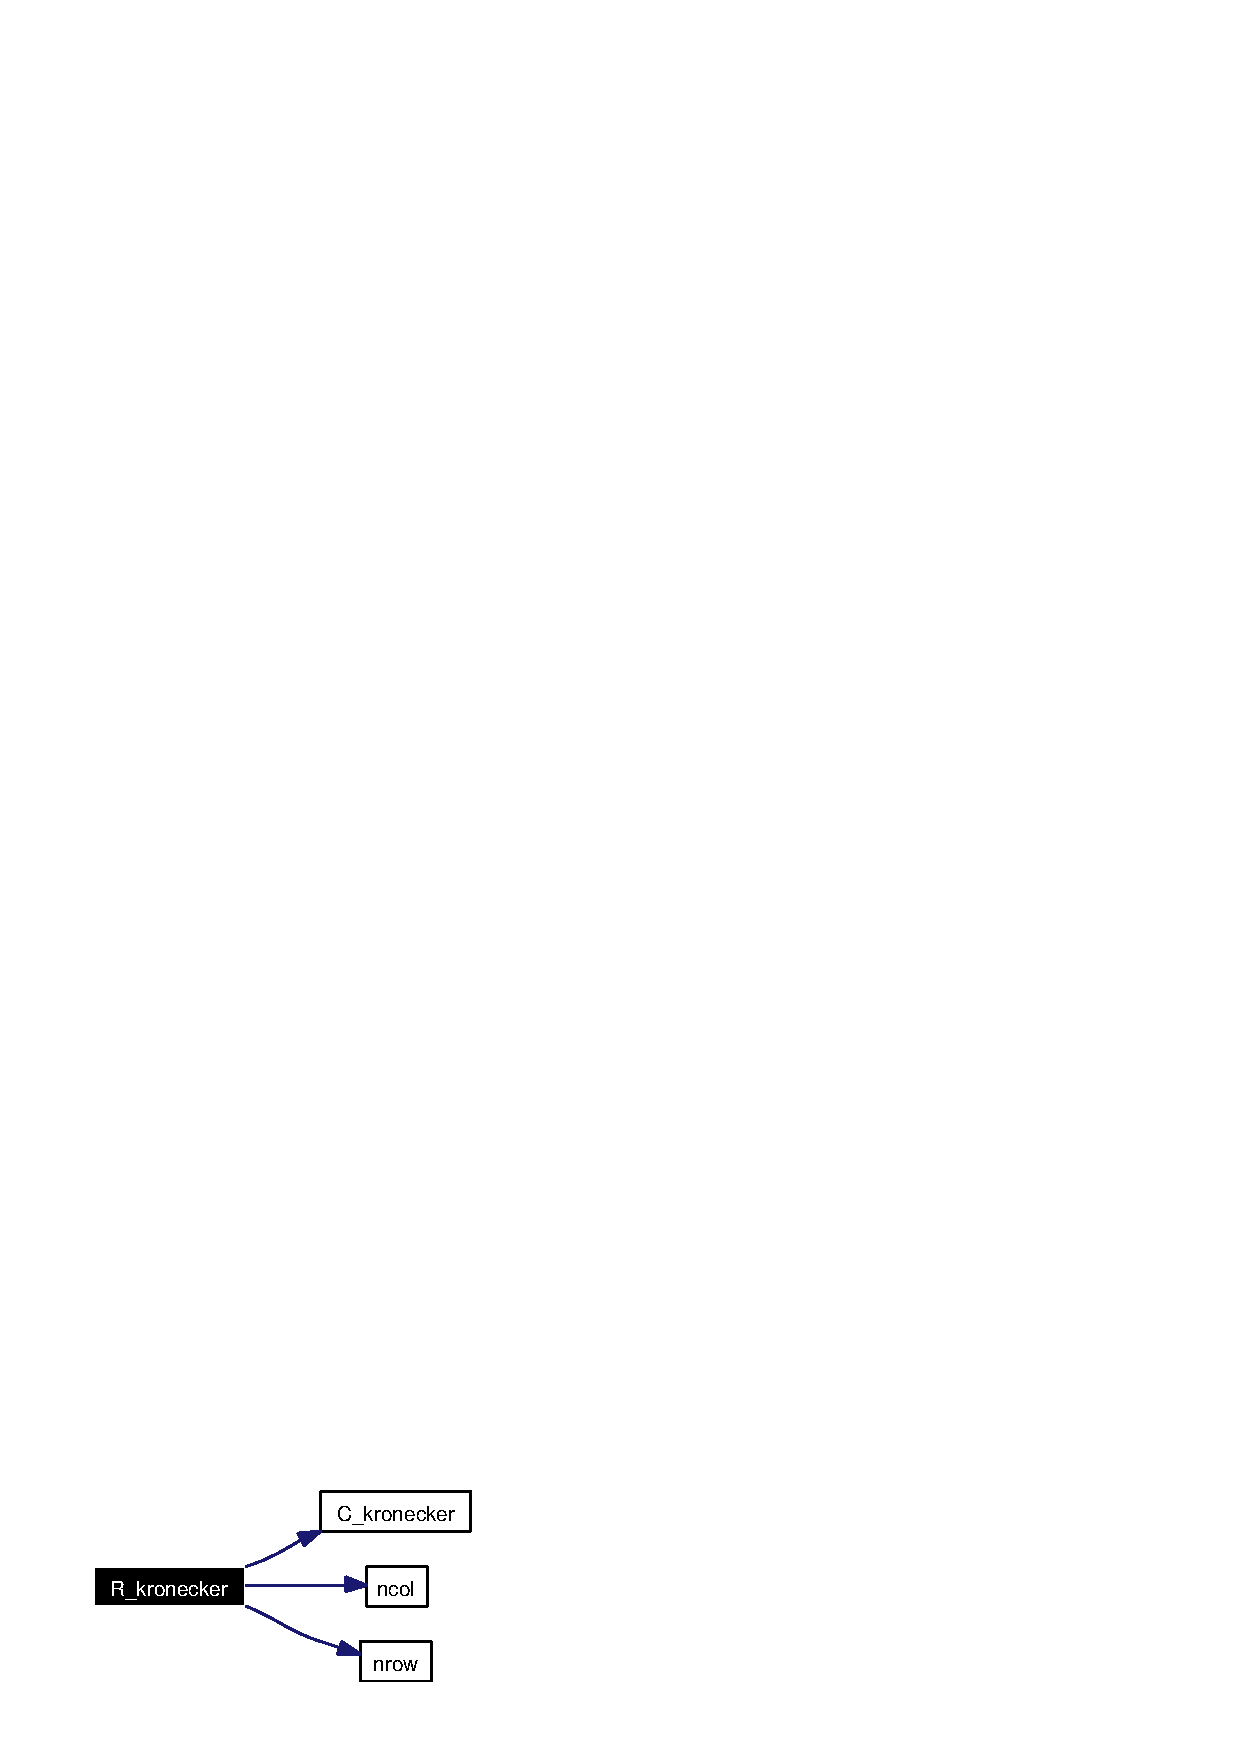
\includegraphics[width=117pt]{LinearStatistic_8c_a1_cgraph}
\end{center}
\end{figure}
\hypertarget{LinearStatistic_8c_a7}{
\index{LinearStatistic.c@{Linear\-Statistic.c}!R_LinearStatistic@{R\_\-LinearStatistic}}
\index{R_LinearStatistic@{R\_\-LinearStatistic}!LinearStatistic.c@{Linear\-Statistic.c}}
\subsubsection[R\_\-LinearStatistic]{\setlength{\rightskip}{0pt plus 5cm}SEXP R\_\-Linear\-Statistic (SEXP {\em x}, SEXP {\em y}, SEXP {\em weights})}}
\label{LinearStatistic_8c_a7}


R-interface to C\_\-Linear\-Statistic \par
 \begin{Desc}
\item[Parameters:]
\begin{description}
\item[{\em x}]values of the transformation \item[{\em y}]values of the influence function \item[{\em weights}]case weights \end{description}
\end{Desc}


Definition at line 363 of file Linear\-Statistic.c.

References C\_\-Linear\-Statistic(), ncol(), and nrow().

Here is the call graph for this function:\begin{figure}[H]
\begin{center}
\leavevmode
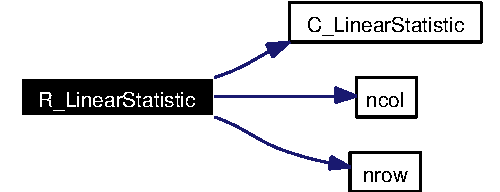
\includegraphics[width=137pt]{LinearStatistic_8c_a7_cgraph}
\end{center}
\end{figure}
\hypertarget{LinearStatistic_8c_a9}{
\index{LinearStatistic.c@{Linear\-Statistic.c}!R_PermutedLinearStatistic@{R\_\-PermutedLinearStatistic}}
\index{R_PermutedLinearStatistic@{R\_\-PermutedLinearStatistic}!LinearStatistic.c@{Linear\-Statistic.c}}
\subsubsection[R\_\-PermutedLinearStatistic]{\setlength{\rightskip}{0pt plus 5cm}SEXP R\_\-Permuted\-Linear\-Statistic (SEXP {\em x}, SEXP {\em y}, SEXP {\em indx}, SEXP {\em perm})}}
\label{LinearStatistic_8c_a9}


Linear Statistic with permuted indices\par
 \begin{Desc}
\item[Parameters:]
\begin{description}
\item[{\em x}]values of the transformation \item[{\em y}]values of the influence function \item[{\em indx}]indices for the x-part \item[{\em perm}](permuted) indices for the y-part \end{description}
\end{Desc}


Definition at line 442 of file Linear\-Statistic.c.

References C\_\-Permuted\-Linear\-Statistic(), ncol(), and nrow().

Here is the call graph for this function:\begin{figure}[H]
\begin{center}
\leavevmode
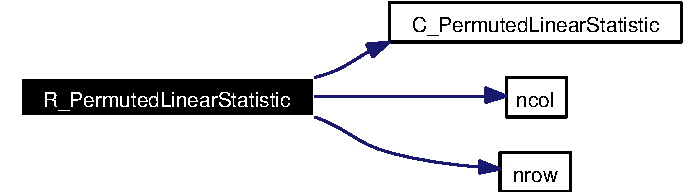
\includegraphics[width=185pt]{LinearStatistic_8c_a9_cgraph}
\end{center}
\end{figure}
\hypertarget{LinearStatistic_8c_a11}{
\index{LinearStatistic.c@{Linear\-Statistic.c}!R_scmatleft@{R\_\-scmatleft}}
\index{R_scmatleft@{R\_\-scmatleft}!LinearStatistic.c@{Linear\-Statistic.c}}
\subsubsection[R\_\-scmatleft]{\setlength{\rightskip}{0pt plus 5cm}SEXP R\_\-scmatleft (SEXP {\em x}, SEXP {\em pq})}}
\label{LinearStatistic_8c_a11}


R-interface to C\_\-scmatleft \begin{Desc}
\item[Parameters:]
\begin{description}
\item[{\em x}]score vector of length p \item[{\em pq}]dimension of the linear statistic \end{description}
\end{Desc}


Definition at line 530 of file Linear\-Statistic.c.

References C\_\-scmatleft().

Here is the call graph for this function:\begin{figure}[H]
\begin{center}
\leavevmode
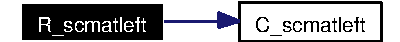
\includegraphics[width=113pt]{LinearStatistic_8c_a11_cgraph}
\end{center}
\end{figure}
\hypertarget{LinearStatistic_8c_a13}{
\index{LinearStatistic.c@{Linear\-Statistic.c}!R_scmatright@{R\_\-scmatright}}
\index{R_scmatright@{R\_\-scmatright}!LinearStatistic.c@{Linear\-Statistic.c}}
\subsubsection[R\_\-scmatright]{\setlength{\rightskip}{0pt plus 5cm}SEXP R\_\-scmatright (SEXP {\em x}, SEXP {\em pq})}}
\label{LinearStatistic_8c_a13}


R-interface to C\_\-scmatright \begin{Desc}
\item[Parameters:]
\begin{description}
\item[{\em x}]score vector of length q \item[{\em pq}]dimension of the linear statistic \end{description}
\end{Desc}


Definition at line 595 of file Linear\-Statistic.c.

References C\_\-scmatright().

Here is the call graph for this function:\begin{figure}[H]
\begin{center}
\leavevmode
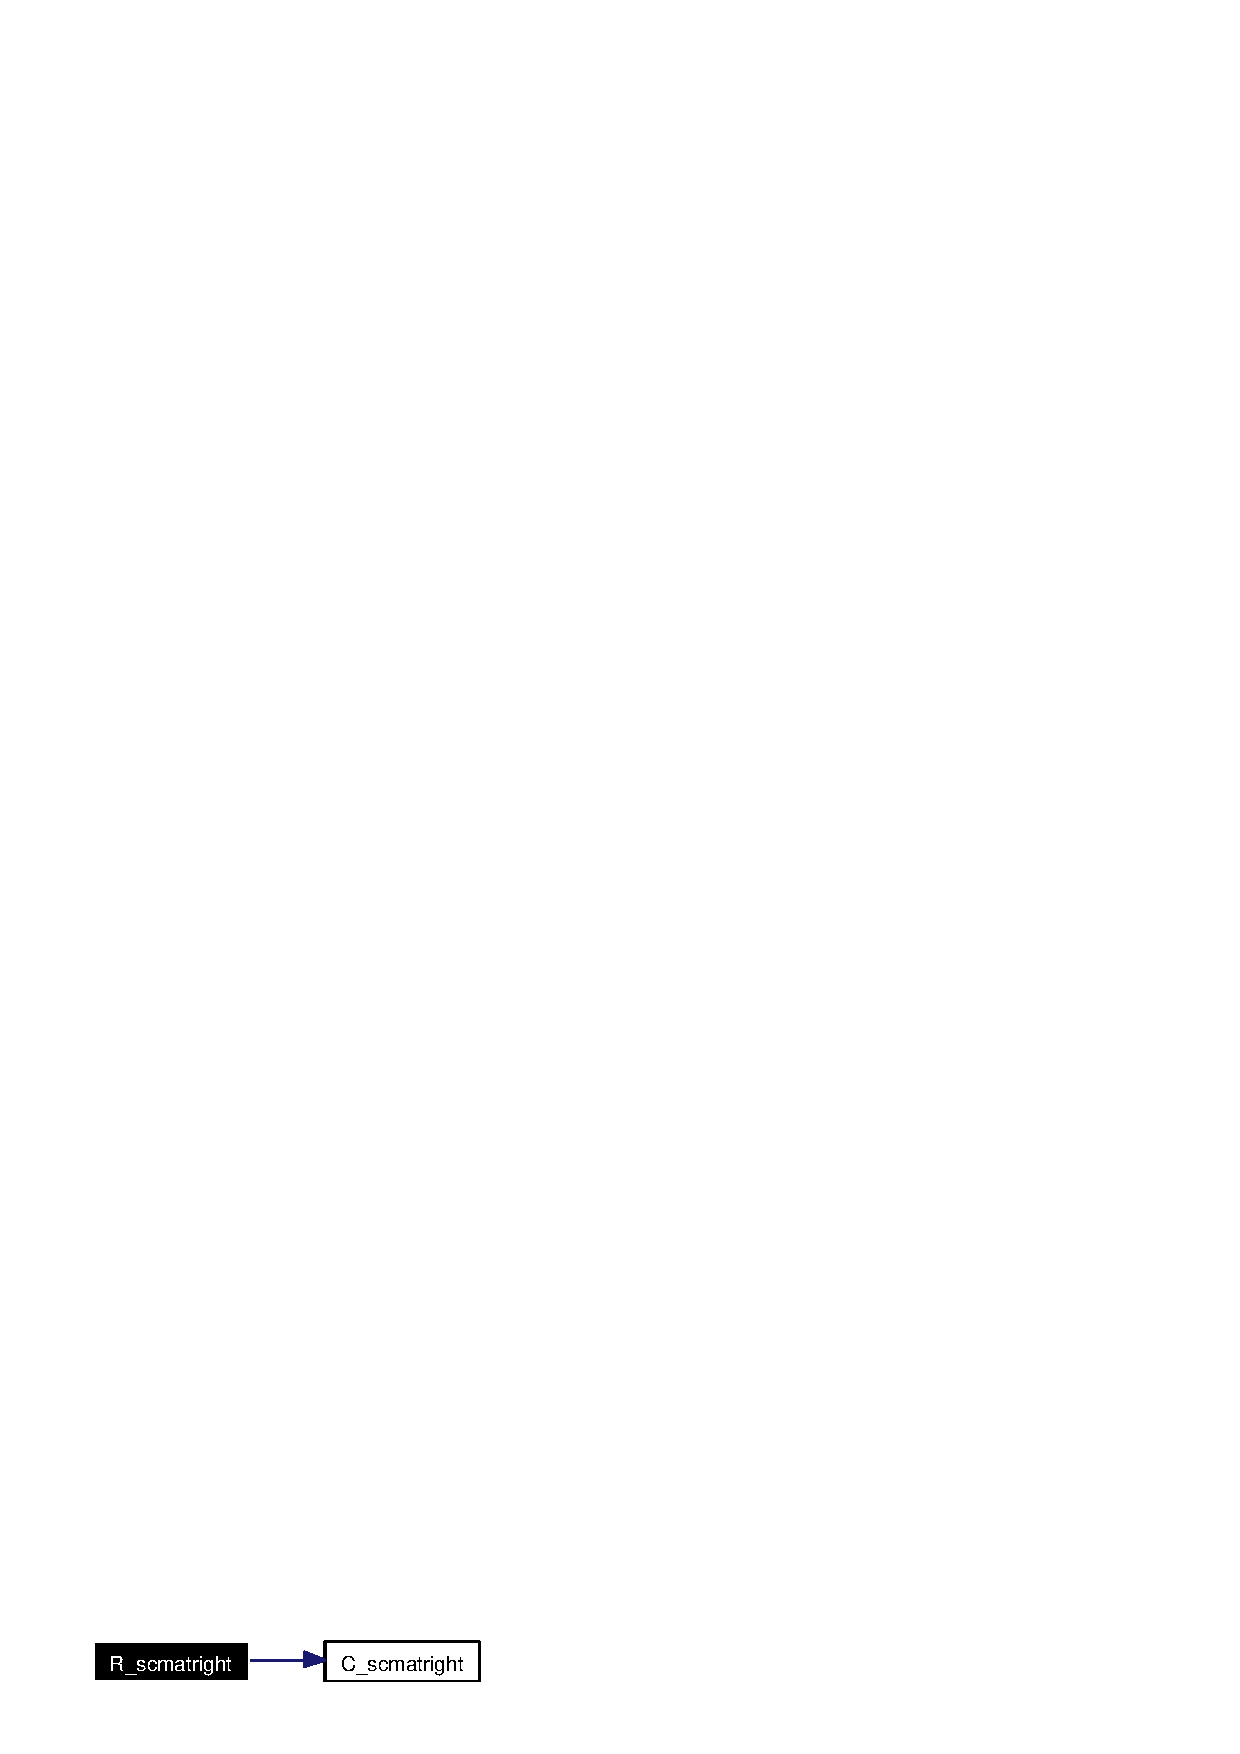
\includegraphics[width=119pt]{LinearStatistic_8c_a13_cgraph}
\end{center}
\end{figure}
